% One cluster's memories (itmn_m2/src/common/Memory_Cluster.v) and the mirror logic of Mamba_Top.v.
\documentclass[tikz,border=4pt]{standalone}
% Shared style of the RTL diagrams. Build one with: tectonic fig_x.tex
\usepackage{tikz}
\usetikzlibrary{arrows.meta,positioning,fit,calc,backgrounds,shapes.geometric}
\usepackage[T1]{fontenc}
\usepackage{lmodern}
% opaque background, so the SVGs stay readable on dark pages
\tikzset{every picture/.append style={show background rectangle,
         background rectangle/.style={fill=white, draw=none}, inner frame sep=2pt}}
\definecolor{inkA}{HTML}{0B0B0B}
\definecolor{inkB}{HTML}{52514E}
\definecolor{rule}{HTML}{C3C2B7}
\definecolor{fillA}{HTML}{F0EFEC}
\definecolor{fillPE}{HTML}{CDE2FB}
\definecolor{fillRow}{HTML}{FBE0D3}
\definecolor{fillMem}{HTML}{E5F4EC}
\definecolor{fillCtl}{HTML}{FDF0C8}
\definecolor{fillReg}{HTML}{F6C9A8}
\definecolor{ctlink}{HTML}{8A6A00}
\tikzset{
  blk/.style={draw=inkB, line width=0.5pt, rounded corners=1.5pt, align=center, font=\scriptsize, inner sep=2pt},
  pe/.style={blk, fill=fillPE},
  row/.style={blk, fill=fillRow},
  mem/.style={blk, fill=fillMem},
  ctl/.style={blk, fill=fillCtl},
  plain/.style={blk, fill=white},
  grp/.style={draw=rule, line width=0.6pt, rounded corners=3pt, inner sep=4pt},
  dgrp/.style={draw=inkB, dashed, line width=0.5pt, rounded corners=3pt, inner sep=4pt},
  arr/.style={-{Stealth[length=3pt]}, line width=0.5pt, draw=inkB},
  darr/.style={{Stealth[length=3pt]}-{Stealth[length=3pt]}, line width=0.5pt, draw=inkB},
  carr/.style={-{Stealth[length=2.5pt]}, line width=0.4pt, draw=ctlink, densely dashed},
  lbl/.style={font=\scriptsize, text=inkB, align=center},
  tlbl/.style={font=\tiny, text=inkB, align=center},
  clbl/.style={font=\tiny, text=ctlink, align=center},
  opc/.style={circle, draw=inkB, fill=white, line width=0.5pt, minimum size=0.42cm, inner sep=0pt, font=\scriptsize},
  mux/.style={trapezium, trapezium stretches=true, trapezium angle=70, draw=inkB, fill=fillA, line width=0.5pt, minimum height=0.38cm,
              inner sep=1pt, font=\tiny, shape border rotate=180},
  regbar/.style={draw=inkB, fill=fillReg, line width=0.5pt, minimum height=0.16cm, inner sep=0pt},
}
% bus width mark: \bw{coordinate}{width}
\newcommand{\bw}[2]{\draw[line width=0.4pt, draw=inkB] ($(#1)+(-0.06,-0.06)$) -- ($(#1)+(0.06,0.06)$)
  node[tlbl, anchor=west, inner sep=1pt] {#2};}

\tikzset{dma/.style={-{Stealth[length=3pt]}, line width=0.5pt, draw=inkB!70, dashed}}
\begin{document}
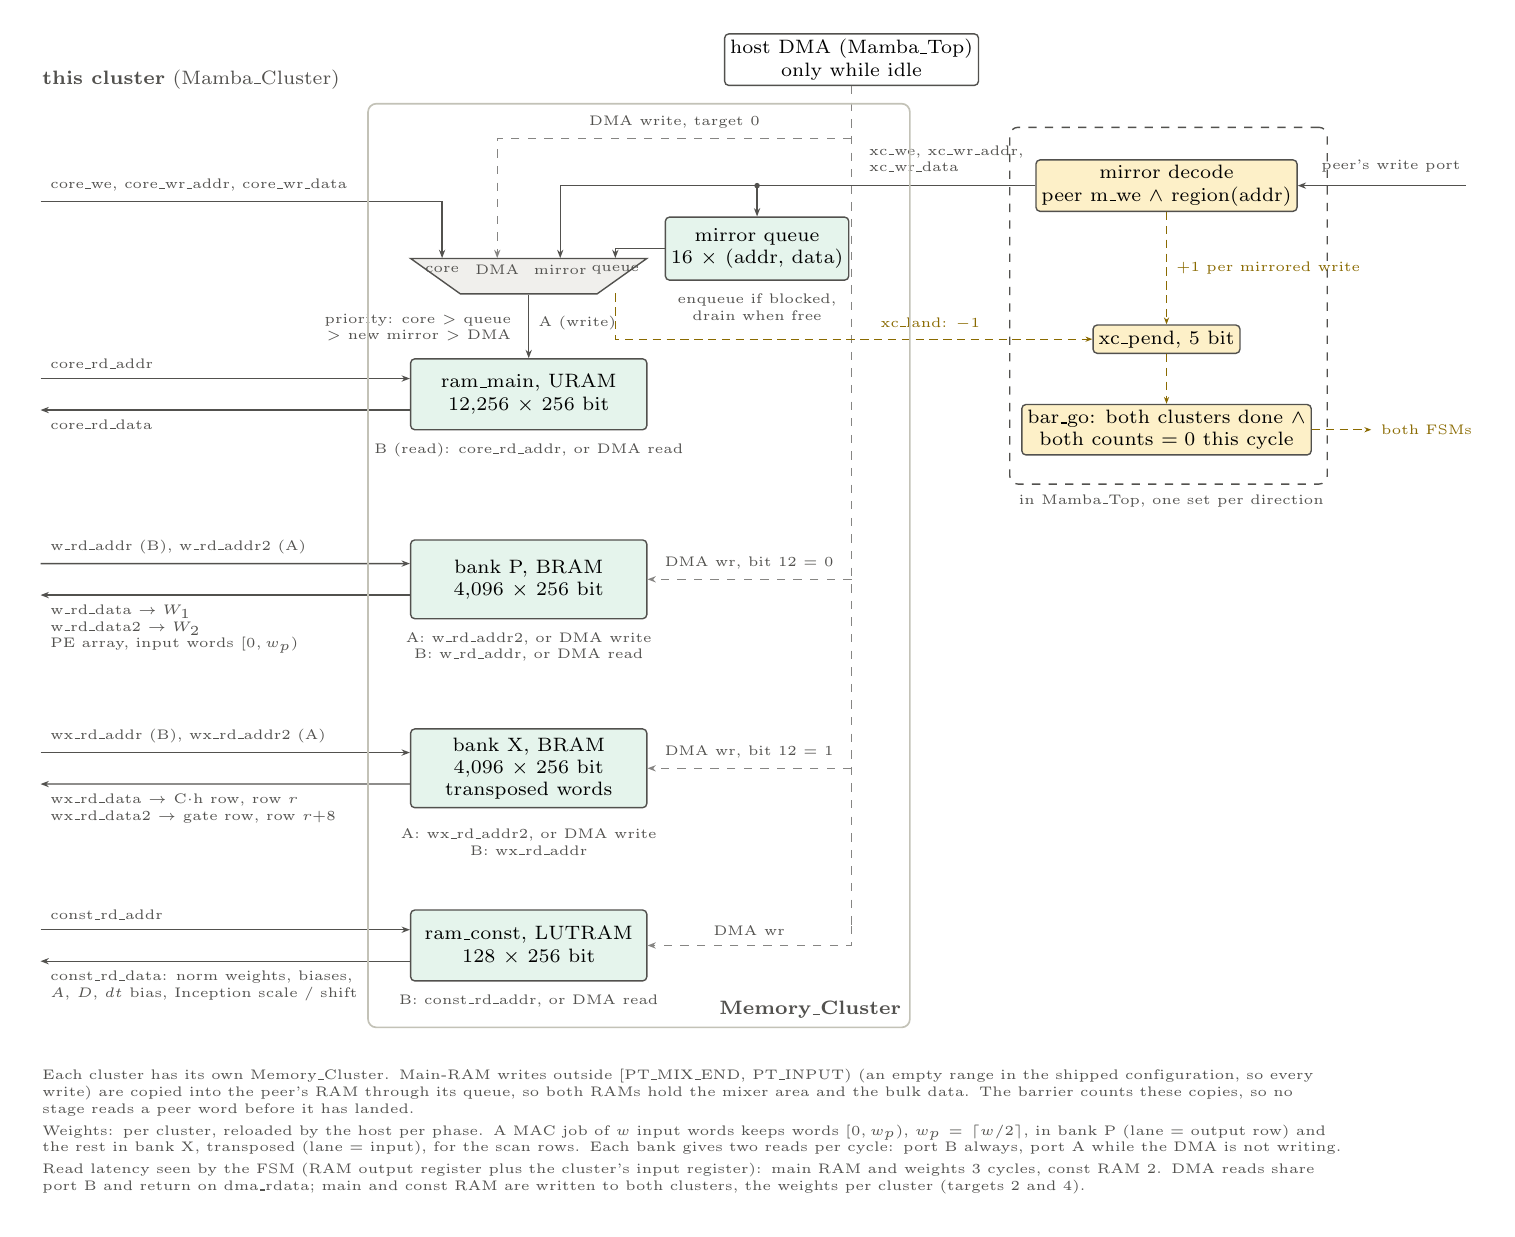
\begin{tikzpicture}[x=1cm,y=1cm]
  % ================================================================ sides
  \node[lbl, anchor=west] at (0.2,13.75) {\textbf{this cluster} (Mamba\_Cluster)};
  \node[plain, minimum width=2.6cm] (dma) at (10.6,14.0) {host DMA (Mamba\_Top)\\only while idle};
  \draw[dma, -] (dma.south) -- (10.6,3.0);

  % ================================================================ main RAM: write arbiter and mirror queue
  \node[mux, minimum width=3.0cm, minimum height=0.45cm] (wmx) at (6.5,11.25) {};
  \foreach \n/\x in {core/5.4, DMA/6.1, mirror/6.9, queue/7.6} {\node[font=\fontsize{4.5}{5}\selectfont, text=inkB] at (\x,11.33) {\n};}
  \draw[arr] (0.3,12.2) -- (5.4,12.2) -- (5.4,11.48);
  \node[tlbl, anchor=south west] at (0.3,12.2) {core\_we, core\_wr\_addr, core\_wr\_data};
  \draw[dma] (10.6,13.0) -- (6.1,13.0) -- (6.1,11.48);
  \node[tlbl, anchor=south] at (8.35,13.0) {DMA write, target 0};
  % mirror decode in Mamba_Top
  \node[ctl] (dec) at (14.6,12.4) {mirror decode\\peer m\_we $\wedge$ region(addr)};
  \draw[arr] (18.4,12.4) -- (dec.east);
  \node[tlbl, anchor=south] at (17.45,12.45) {peer's write port};
  \draw[arr] (dec.west) -- (6.9,12.4) -- (6.9,11.48);
  \node[tlbl, anchor=south west, align=left] at (10.7,12.45) {xc\_we, xc\_wr\_addr,\\xc\_wr\_data};
  \node[mem, minimum width=2.0cm, minimum height=0.8cm] (q) at (9.4,11.6) {mirror queue\\16 $\times$ (addr, data)};
  \draw[arr] (9.4,12.4) -- (q.north);
  \fill[inkB] (9.4,12.4) circle (0.035);
  \draw[arr] (q.west) -- (7.6,11.6) -- (7.6,11.48);
  \node[tlbl, anchor=north, align=center] at (9.4,11.15) {enqueue if blocked,\\drain when free};
  \node[mem, minimum width=3.0cm, minimum height=0.9cm] (rm) at (6.5,9.75) {ram\_main, URAM\\12,256 $\times$ 256 bit};
  \draw[arr] (wmx.south) -- (rm.north) node[tlbl, pos=0.45, right] {A (write)};
  \node[tlbl, anchor=east, align=right] at (6.4,10.6) {priority: core $>$ queue\\$>$ new mirror $>$ DMA};
  \draw[arr] (0.3,9.95) -- ($(rm.west)+(0,0.2)$);
  \node[tlbl, anchor=south west] at (0.3,9.95) {core\_rd\_addr};
  \draw[arr] ($(rm.west)+(0,-0.2)$) -- (0.3,9.55);
  \node[tlbl, anchor=north west] at (0.3,9.55) {core\_rd\_data};
  \node[tlbl, anchor=north] at (6.5,9.25) {B (read): core\_rd\_addr, or DMA read};
  % mirrored-write count and the barrier
  \node[ctl] (cnt) at (14.6,10.45) {xc\_pend, 5 bit};
  \draw[carr] (7.6,11.03) -- (7.6,10.45) -- (cnt.west);
  \node[clbl, anchor=south] at (11.6,10.45) {xc\_land: $-1$};
  \draw[carr] (dec.south) -- (cnt.north) node[clbl, pos=0.5, right] {$+1$ per mirrored write};
  \node[ctl] (bar) at (14.6,9.3) {bar\_go: both clusters done $\wedge$\\both counts $= 0$ this cycle};
  \draw[carr] (cnt.south) -- (bar.north);
  \draw[carr] (bar.east) -- (17.2,9.3) node[clbl, anchor=west] {both FSMs};
  \node[dgrp, fit={(12.75,13.0) (16.5,8.75)}] (top) {};
  \node[tlbl, anchor=north west] at (top.south west) {in Mamba\_Top, one set per direction};

  % ================================================================ weight banks
  \node[mem, minimum width=3.0cm, minimum height=1.0cm] (bp) at (6.5,7.4) {bank P, BRAM\\4,096 $\times$ 256 bit};
  \draw[arr] (0.3,7.6) -- ($(bp.west)+(0,0.2)$);
  \node[tlbl, anchor=south west] at (0.3,7.6) {w\_rd\_addr (B), w\_rd\_addr2 (A)};
  \draw[arr] ($(bp.west)+(0,-0.2)$) -- (0.3,7.2);
  \node[tlbl, anchor=north west, align=left] at (0.3,7.2) {w\_rd\_data $\to W_1$\\w\_rd\_data2 $\to W_2$\\PE array, input words $[0, w_p)$};
  \draw[dma] (10.6,7.4) -- (bp.east);
  \node[tlbl, anchor=south] at (9.3,7.4) {DMA wr, bit 12 = 0};
  \node[tlbl, anchor=north, align=center] at (6.5,6.85) {A: w\_rd\_addr2, or DMA write\\B: w\_rd\_addr, or DMA read};

  \node[mem, minimum width=3.0cm, minimum height=1.0cm] (bx) at (6.5,5.0) {bank X, BRAM\\4,096 $\times$ 256 bit\\transposed words};
  \draw[arr] (0.3,5.2) -- ($(bx.west)+(0,0.2)$);
  \node[tlbl, anchor=south west] at (0.3,5.2) {wx\_rd\_addr (B), wx\_rd\_addr2 (A)};
  \draw[arr] ($(bx.west)+(0,-0.2)$) -- (0.3,4.8);
  \node[tlbl, anchor=north west, align=left] at (0.3,4.8) {wx\_rd\_data $\to$ C$\cdot$h row, row $r$\\wx\_rd\_data2 $\to$ gate row, row $r{+}8$};
  \draw[dma] (10.6,5.0) -- (bx.east);
  \node[tlbl, anchor=south] at (9.3,5.0) {DMA wr, bit 12 = 1};
  \node[tlbl, anchor=north, align=center] at (6.5,4.35) {A: wx\_rd\_addr2, or DMA write\\B: wx\_rd\_addr};

  % ================================================================ const RAM
  \node[mem, minimum width=3.0cm, minimum height=0.9cm] (rc) at (6.5,2.75) {ram\_const, LUTRAM\\128 $\times$ 256 bit};
  \draw[arr] (0.3,2.95) -- ($(rc.west)+(0,0.2)$);
  \node[tlbl, anchor=south west] at (0.3,2.95) {const\_rd\_addr};
  \draw[arr] ($(rc.west)+(0,-0.2)$) -- (0.3,2.55);
  \node[tlbl, anchor=north west, align=left] at (0.3,2.55) {const\_rd\_data: norm weights, biases,\\$A$, $D$, $dt$ bias, Inception scale / shift};
  \draw[dma] (10.6,3.0) |- (rc.east);
  \node[tlbl, anchor=south] at (9.3,2.75) {DMA wr};
  \node[tlbl, anchor=north] at (6.5,2.25) {B: const\_rd\_addr, or DMA read};

  \node[grp, fit={(4.6,13.3) (11.2,1.85)}] (mc) {};
  \node[lbl, anchor=south east] at (mc.south east) {\textbf{Memory\_Cluster}};

  % ================================================================ notes
  \node[tlbl, anchor=north west, align=left, text width=16.5cm] at (0.2,1.3) {%
    Each cluster has its own Memory\_Cluster. Main-RAM writes outside $[$PT\_MIX\_END, PT\_INPUT$)$ (an empty range in
    the shipped configuration, so every write) are copied into the peer's RAM through its queue, so both RAMs hold
    the mixer area and the bulk data. The barrier counts these copies, so no stage reads a peer word before it
    has landed.\\[2pt]
    Weights: per cluster, reloaded by the host per phase. A MAC job of $w$ input words keeps words $[0, w_p)$,
    $w_p = \lceil w/2 \rceil$, in bank P (lane = output row) and the rest in bank X, transposed (lane = input), for
    the scan rows. Each bank gives two reads per cycle: port B always, port A while the DMA is not writing.\\[2pt]
    Read latency seen by the FSM (RAM output register plus the cluster's input register): main RAM and weights 3
    cycles, const RAM 2. DMA reads share port B and return on dma\_rdata; main and const RAM are written to both
    clusters, the weights per cluster (targets 2 and 4).};
\end{tikzpicture}
\end{document}
